\documentclass[12pt,letterpaper]{article}
\usepackage{natbib}

%Packages
\usepackage{textcomp}
\usepackage{fullpage}
\usepackage{float}
\usepackage{latexsym}
\usepackage{url}
\usepackage{epsfig}
\usepackage{graphicx}
\usepackage{amssymb}
\usepackage{amsmath}
\usepackage{mathtools}
\usepackage{bm}
\usepackage{array}
\usepackage[version=3]{mhchem}
\usepackage{ifthen}
\usepackage{caption}
\usepackage{hyperref}
\usepackage{amsthm}
\usepackage{amstext}
\usepackage{enumerate}
\usepackage[osf]{mathpazo}
\usepackage{dcolumn}
\usepackage{lineno}
\usepackage{pdflscape}

\usepackage{color,soul}

\DeclarePairedDelimiter\abs{\lvert}{\rvert}%
\DeclarePairedDelimiter\norm{\lVert}{\rVert}%
\newcolumntype{d}[1]{D{.}{.}{#1}}

\pagenumbering{arabic}


%Pagination style and stuff
\linespread{2}
\raggedright
\setlength{\parindent}{0.5in}
\setcounter{secnumdepth}{0} 
\renewcommand{\section}[1]{%
\bigskip
\begin{center}
\begin{Large}
\normalfont\scshape #1
\medskip
\end{Large}
\end{center}}
\renewcommand{\subsection}[1]{%
\bigskip
\begin{center}
\begin{large}
\normalfont\itshape #1
\end{large}
\end{center}}
\renewcommand{\subsubsection}[1]{%
\vspace{2ex}
\noindent
\textit{#1.}---}
\renewcommand{\tableofcontents}{}
%\bibpunct{(}{)}{;}{a}{}{,}

%---------------------------------------------
%
%       START
%
%---------------------------------------------

\begin{document}
%Running head
\begin{flushright}
Version dated: \today
\end{flushright}

\bigskip
\noindent RH: disparate disparity analyses
\bigskip
\medskip
\begin{center}
\noindent{\Large \bf Disparities in the analysis of morphological disparity}
\bigskip

Thomas Guillerme$^{1,16,*,+}$,
Natalie Cooper$^{2,+}$,
Stephen L. Brusatte$^{3}$,
Katie E. Davis$^{4}$,
Andrew L Jackson$^{5}$,
Sylvain Gerber$^{6}$,
Anjali Goswami$^{2}$,
Kevin Healy$^{7}$,
Melanie Hopkins$^{8}$,
Marc EH Jones$^{9}$,
Graeme T. Lloyd$^{10}$,
Joseph E. O'Reilly$^{11}$,
Abi Pate$^{11}$,
Mark N Puttick$^{12}$,
Emiliy Rayfield$^{11}$,
Erin E. Saupe$^{13}$,
Emma Sherratt$^{14}$,
Graham Slater$^{15}$,
Vera Weisbecker$^{1}$,
Gavin H Thomas$^{16}$
and Philip Donoghue$^{11}$\\


\noindent {\small \it 
$^1$School of Biological Sciences, University of Queensland, St. Lucia, Queensland, Australia;
$^2$IDepartment of Life Sciences, Natural History Museum, London, Cromwell Road, London, SW7 5BD, UK;
$^{3}$School of GeoSciences, University of Edinburgh, Grant Institute, Edinburgh EH9 3FE, UK;
$^{4}$Department of Biology, University of York, YO10 5DD, UK;
$^{5}$Department of Zoology, School of Natural Sciences, Trinity College, Ireland;
$^{6}$Institut de Syst\'{e}matique, \'{E}volution, Biodiversit\'{e} (ISYEB), Muséum national d'Histoire naturelle, CNRS, Sorbonne Universit\'{e}, EPHE, Université des Antilles, 57 rue Cuvier CP39, 75005 Paris, France;
$^{7}$Ryan Institute, School of Natural Sciences, National University of Ireland Galway, Ireland;
$^{8}$ @@@;
$^{10}$School of Earth and Environment, University of Leeds, Leeds LS2 9JT, UK;
$^{11}$School of Earth Sciences, University of Bristol, Life Sciences Building, Tyndall Avenue, Bristol BS8 1TQ, UK;
$^{12}$Milner Centre for Evolution, University of Bath, BA2 7AY UK;
$^{13}$Department of Earth Sciences, University of Oxford, S Parks Road, Oxford OX1 3AN, UK;
$^{14}$School of Biological Sciences, The University of Adelaide, Adelaide, South Australia 5005, Australia.
$^{15}$ @@@;
$^{16}$ @@@;\\
$^{+}$ These authors contributed equally to the manuscript; $^{*}$ Corresponding author: guillert@tcd.ie\\}

\end{center}

\textbf{Abstract (200 words max)}

\noindent Analyses of morphological disparity have been used to characterise and investigate the evolution of variation in the anatomy, function, and ecology of organisms since the 1980s.
While a diversity of methods have been employed, it is unclear whether they provide
equivalent insights.
Here we review the most commonly used approaches for characterising and analysing morphological disparity, all of which have associated limitations that, if ignored, can lead to misinterpretation.
We provide best practice guidelines for disparity analyses, while noting that there can be no ``one-size-fits-all'' approach.
The available tools should always be used in the context of a specific biological question that will determine data and method selection at every stage of the analysis.

\textbf{Keywords}: multidimensionality, palaeobiology, ecology,
morphology, disparity, variance/variation

\section{Introduction}

%@@@ add links to figures

\noindent Clades of organisms are characterised by variation in both numbers of species and range of phenotypes through time.
At the extremes, clades may be exceptionally species-rich and phenotypically diverse (e.g. cichlids and molluscs), species-rich but phenotypically conservative (e.g. bacteria and nematodes), species-poor but phenotypically diverse (e.g. Afrotheria), or depauperate in both species and phenotypic diversity (e.g. lungfish).
These phenomena suggest that taxonomic and phenotypic diversity are not inextricably linked, raising important questions about how phenotypic diversity arises, such as:
How does diversity evolve?
Are some morphologies more common than others?
Can anatomy evolve in all ``directions'' or are some anatomies impossible to achieve? (Mike Foote 1997, 1995)
What role does ecology play in structuring morphological diversity?
Analyses of species diversity have a venerable history, but those of phenotypic diversity (hereafter \emph{disparity}) are a comparatively more recent phenomenon. Originally defined as ``multidimensional morphological dissimilarity at a macroevolutionary scale'' \citep{runnegar1987rates,Gould1991-nh} this concept of disparity emerged from attempts by palaeobiologists to characterise the evolutionary origin of animal bodyplans and from attempts by comparative developmental biologists to provide causal explanations for their emergence.
However, analyses of ``disparity'' have since expanded into comparative biology as a means of capturing the effect of intrinsic and extrinsic causal agents in morphological evolution.
Typically, methods to capture disparity are based on multidimensional spaces where each dimension represents an aspect of morphological variation (a trait) and biological observations (taxa) can be placed in this space based on their trait values.
Such multidimensional spaces (or morphospaces) can then be used to tackle a diverse array of questions that can be grouped into four main (non-mutually exclusive) classes (Fig. 1):

\begin{enumerate}

	\item \textbf{Descriptive disparity} The pioneering studies of disparity characterised the shapes of organisms and how they differed among groups \citep{Foote1995-do, Briggs1992-pd}.
	These studies consist of describing multidimensional patterns in the diversity of morphological traits, addressing questions such as: why are some morphological trait combinations more common than others and what are the biological (or mathematical) properties of the resulting morphospace? \citep{Foote1995-do, Raup1961-vx, Gerber2017-xi}.

	\item \textbf{Disparity-through-time} This approach investigates how the morphologies of organisms have changed on a temporal scale, focussing on the disparity of taxa in particular time intervals or slices.
	This approach has been used widely in palaeobiology to answer a range of macroevolutionary questions, such as: how does disparity accumulate over the history of a clade \citep{Guillerme2018-uj, Wright2017-jo}, or how does disparity change leading up to and across mass extinction events \citep{Friedman2010-ve}?

	\item \textbf{Disparity and taxonomic diversity} Morphological disparity provides another perspective on biodiversity; high morphological disparity represents a high diversity of morphologies (i.e. shapes or body plans) and is, presumably, associated with high levels of ecological and functional diversity (though see section 4 below).
	This makes disparity an informative complement to diversity measures based on species richness alone. Indeed, most studies that have investigated disparity and taxonomic diversity support an effective decoupling 
	\citep[e.g.][]{Fortey1996-kt, Moyne2007-jm, Ruta2013-iy, Hopkins2013-xt}.
	This approach has been used to investigate whether some groups are more successful than others in their exploration of new evolutionary strategies \citep{Losos2011-fq}.

	\item \textbf{Disparity as a proxy for ecology} The disparity of a group can be used as a proxy for either the functional role it plays within an ecosystem or its ecological niche.
	This approach assumes that groups with high disparity are also likely to be functionally and ecologically diverse, and that groups found in similar regions of shape space will have similar functional and ecological roles
	\citep{Friedman2010-ve, Pierce2008-yr, Anderson2013-zt}.
	The links between form and function, however, are not always clear cut.
	Traits can be linked to multiple functions and multiple functions can be linked to a single trait \citep{Wainwright2005-or}.
	This approach has been used to investigate hypotheses of competitive replacement \citep{Brusatte2008-vx} and changes in ecosystem function during and after mass extinctions \citep{Friedman2010-ve}.
	It is particularly common in palaeobiology where it is not possible to directly observe the ecological or functional characteristics of extinct species \citep{Wainwright2005-or}.

	\item \textbf{Disparity and evo-devo} Morphological disparity blalbalbal
% AG: Although intrinsic constraints are mentioned earlier, it doesn’t enter into any of these topics explicitly, but it is certainly one of the most interesting things one can use disparity for – to bridge development and evolution, looking at developmental biases/constraints. This also includes integration and modularity, which are also central to the topic of disparity and evolvability. Although you touch on these in places, I think it's really important to incorporate it into one of these topics, as there probably isn't room to give it one of its own (although i would argue it warrants equal footing with ecology, given that these are the processes that generate variation in the first place). There is a massive literature on using disparity to test hypotheses of developmental constraints, and also a huge one on disparity and integration/modularity. Let me know if you want me to send you refs.

\end{enumerate}

Fundamental insights into evolutionary biology have been elicited from these five types of analysis.
One of the most important insights is the discovery that morphological disparity is often greatest early in the evolutionary history of clades \citep{Foote1997-nl, Erwin2007-jz, Hughes2013-td}, indicating that the capacity for evolutionary innovation wanes with clade age, which some have argued reflects the evolutionary assembly of gene regulatory networks that constrain later fundamental change  \citep{Erwin2007-jz, Hughes2013-td}.
However, this example highlights one of the most challenging problems confronting researchers who are attempting, increasingly, to obtain general insights from multiple independent studies: can the insights gained from studies using the diversity of methods, approaches and data types employed be considered equivalent?

In attempting to answer this question, we review current methods and highlight their limitations, as part of a more general attempt to propose best practice guidelines for studies of disparity.
We first discuss the appropriate data required for characterising disparity, then review various challenging aspects of these approaches.
Throughout, it is important to remember these tools should always be used in the context of a specific scientific question, as this will drive data and methodological choices at every stage of the process.

\begin{figure}[!htbp]
\centering
   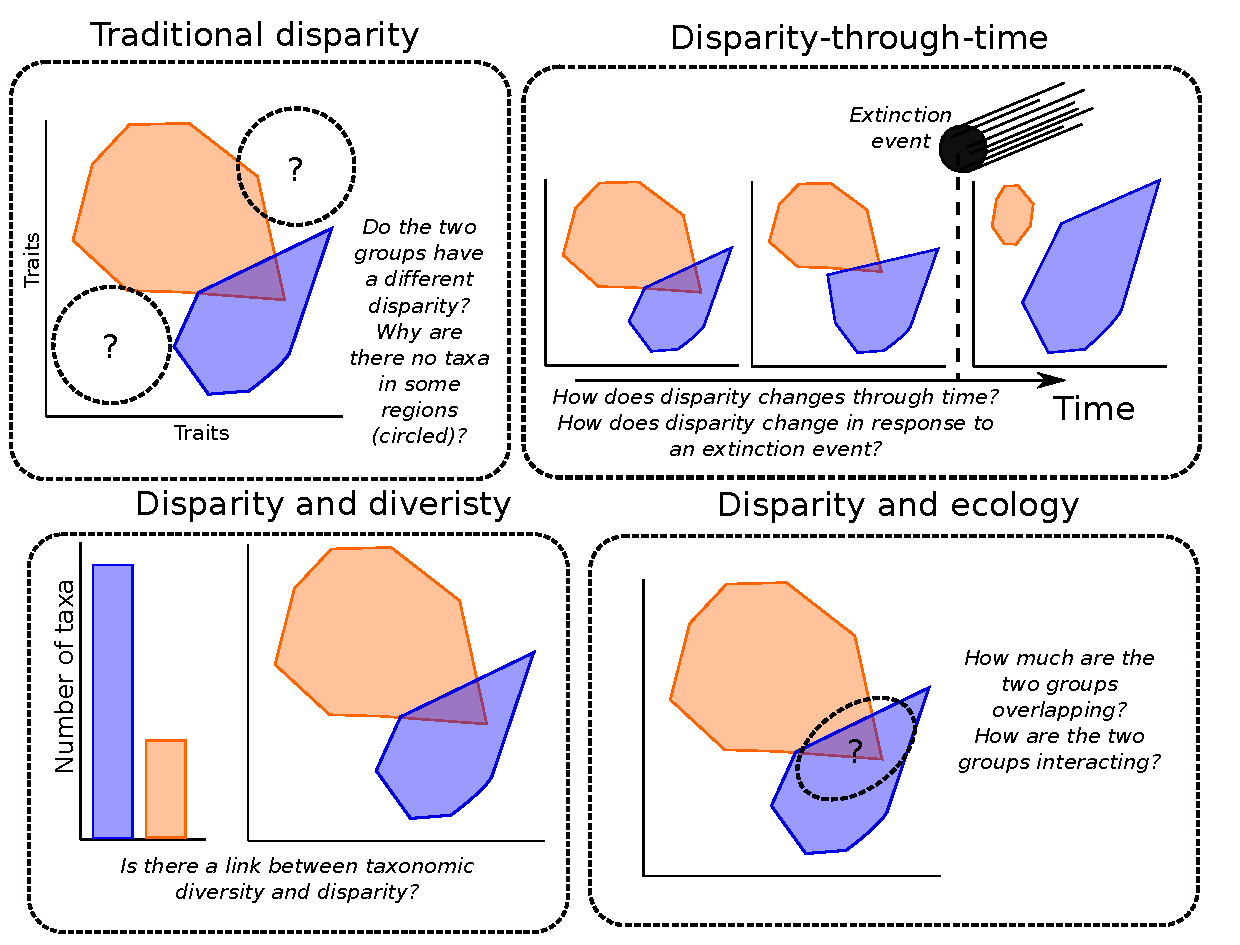
\includegraphics[width=0.9\textwidth]{Figures/figure_disparities.pdf}
\caption{
    The four main types of disparity analysis. \textbf{Descriptive disparity} focuses on describing the features of morphospace occupation; \textbf{disparity-through-time} investigates the evolution of the morphospace through time including the effect of extinction events; \textbf{disparity and taxonomic diversity} compares different measures of biodiversity ; \textbf{disparity as a proxy for ecology} uses disparity as a proxy for the ecological or functional role of a group.
    These categories are not independent and many disparity studies will cover more than one.
    %@@@ Add disparity and evo-devo
}
\label{Fig:disparity}
\end{figure}



\section{Data and disparity}

\noindent Disparity analyses are based on traits, but traits can be characterised in a number of ways:
% MH: We do not mention model-based descriptors at all, or the spaces defined by them (e.g. Raup's shell coiling models). I'm not convinced that we must, but it may come across as an notable omission to reviewers
% SG: I agree. There's for instance Saunders et al. (2004) disparity study of Paleozoic ammonoids using Raup's shell coiling parameters
	1) discrete ``cladistic'' characters, e.g. coding the absence or presence of features or a discrete characteristic of a trait \citep[][e.g]{Close2015-qi};
	2) continuous measurements of features (e.g., lengths) \citep[][e.g]{Anderson2001-qb}; or
	3) more mathematical descriptors from geometric morphometric landmark data (e.g. Procrustes coordinates) \citep[][e.g]{Cooney2017-ly}, and Fourier coefficients \citep[][e.g]{Foote1995-do, Spriggs2018-nu} (Fig. 2).
None of these approaches are superior, but they may be more or less well-suited to characterising traits under comparison and to the question being asked of those traits \citep{hetherington2015cladistic,Hopkins2017-cf}.


For example, if investigating variation of bat wing shapes, both homologous landmarks and continuous measurements of bones may be appropriate to capture patterns of wing variation.
However, if the question focuses on comparing wings between bats and birds, different measurements might be more appropriate depending on the specific question: for example if the focus is on wing function, i.e. whether the aerodynamic properties of wings vary within bats or between bats and birds, the traits collected should reflect these aerodynamic properties (e.g. wingspan, aspect ratio, etc.).
However, if the focus is on convergence between different bats and birds, it would be preferable to use traits that have facilitated flight in both groups (e.g. digit length, integumentary system, etc.).
Where there is any doubt about the appropriate traits to choose, it may be preferable to use different kinds of data for the same feature to determine whether they capture the same pattern of disparity.

The points above assume that researchers are collecting their own data for disparity analyses, but often this is not the case.
Discrete character data are commonly recycled from phylogenetic studies \citep[][e.g]{Foote1989-fd, Deline2018-le}.
% SG: Foote (1989) is a study of trilobite disparity from Fourier analysis of cranidia. I don't think it has anything to do with discrete data or phylogenetic studies
% MH: Also the Foote papers that used discrete data weren't taken from phylogenetic studies but collected for the specific purpose of the project -- I think this might be true for the Deline paper as well. But there are many studies out there that used matrices initially intended for phylogenetics. I can look for some if needed.
This is an efficient approach to character sampling, but it may artifactually increase disparity between phylogenetically distinct groups because phylogenetic characters are often collected to discriminate among groups \citep{Foote1995-do}.
This needs to be considered when interpreting results, especially as synapomorphies will naturally lead to an apparent shift or increase in disparity when new clades appear.
Furthermore, many datasets are limited to subsets of anatomy that are at least implicit samples of overall anatomy, but explicit tests of this assumption have shown that different aspects of morphology can exhibit different patterns of disparity \citep{Hopkins2017-cf}.
This effect of anatomical part on disparity patterns can be especially challenging when working on datasets where the available data has non-random missing anatomical parts, such as the absence of soft tissue in the fossil record \citep{Deline2018-le}.

Trait data suffer from the same shortcomings as most biological datasets -- data can be missing, non-overlapping, hierarchical, inapplicable, ambiguous, polymorphic, correlated, or there may be an insufficient sample size \citep{Brazeau2017-kg, Palci2018-ni}.
Biological phenomena such as allometry and sexual dimorphism may also influence trait data.
More mundanely, data collection is constrained by the time and money available, making collating a ``perfect'' dataset difficult.
Ultimately, disparity analyses characterise the data, and subsamples of the universe of possible data may not have the power to uncover holistic patterns of disparity.
Therefore, trait data should be collected with the question in mind, or the question asked should be tailored to the limits of the data available.

\begin{figure}[!htbp]
\centering
   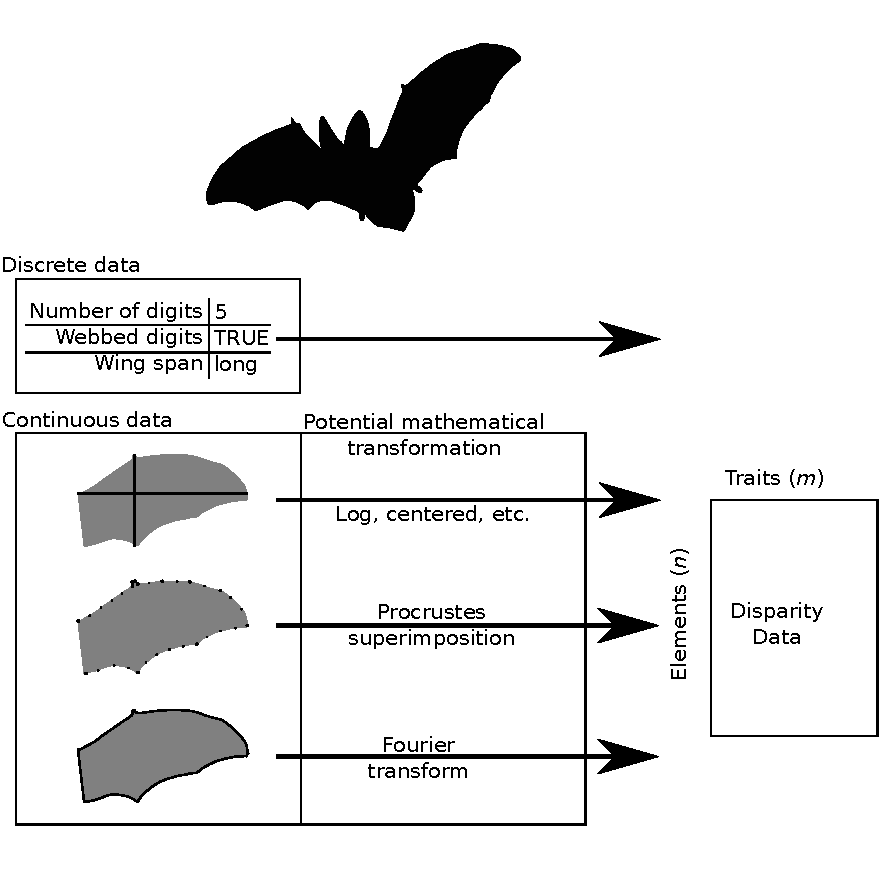
\includegraphics[width=0.9\textwidth]{Figures/figure_data.pdf}
\caption{
    Major routes to obtain morphological data for disparity analyses. Data can be collected as discrete trait observations (e.g. presence or absence data) or as continuous data.
    Continuous data can be collected by various methods including linear measurements and landmark coordinates or contours (curves).
    These measurements can then be mathematically transformed (logarithm transforms, scaling, Procrustes superimposition, elliptic Fourier transforms, etc.).
    Regardless of the method, data collection produces a trait matrix where the observed traits constitute columns and the studied elements (generally taxa or OTUs) the rows.
}
\label{Fig:data}
\end{figure}


\subsection{From data to morphospace}

The concept of what the morphospace \textit{is} can be different between authors and studies but generally used in the common (i.e. non-mathematical) sense of a space containing all possible morphologies.
For the purpose of this review, we use a generalised version of the definition of \cite{mitteroecker2009concept} where the morphospace is a \textit{p}-dimensional space (or Q-space) containing \textit{n} points \citep{mitteroecker2009concept}.
In other words, mathematically, the morphospace is the mathematical object that contains the trait values (\textit{p}, the axes of the space) for all the observations (\textit{n}, the specimens); or, biologically, the morphospace contains all the observed combination of traits.
We generalise this definition to any linear transformation ($V \to W$) of this space that retains the biological definition, i.e. the morphospace is the mathematical object that contains the observed combinations of traits or their transformation.
Note that here the morphospace does not need to be Euclidean (although this is often desired or assumed - see discussion below). %link
If the morphospace is transformed mathematically (i.e. the dataset is transformed using logs, ordinations, distance matrices, etc...) it remains the morphospace as long as all the observation and traits remain in the datatset.

% This generalised definition that we will used throughout the manuscript considers to be a morphospace any mathematical object that contains all the traits and all the observation.
% For example, the raw trait matrix is a morphospace, the distance matrix obtained from that one is the same morphospace, the ordination of that latter is the same morphospace, etc (again, properties of the space can change as long as all the traits and observations are used).
% But if a space is comprised of 95\% of the axes of a PCA, this is not a morphospace anymore but a subset of it.


\section{Disparity analysis methods}

\noindent Once suitable trait data have been collected, the design of the disparity analysis itself needs to be considered.
Study design encompasses several key aspects including (a) the difficulty of dealing with multidimensional data; (b) the indices used to summarise the relative disparity of groups; (c) the methods used for hypothesis testing within the disparity analysis framework; and (d) ancestral state estimations in disparity-through-time analyses.
We consider these aspects in turn below.

\subsection{(a) To ordinate or not to ordinate - that is the (multidimensional) question}

Disparity analyses often use ordination techniques for dimension reduction.
Ordinations are statistical methods to rearrange observed variables so that similar observations are closer together than dissimilar ones (e.g. principal component analysis - PCA; principal coordinates analysis - PCO/PCoA; non-metric multidimensional scaling - NMDS; etc.).
They come in many flavours depending on the data and the desired morphospace properties.
For example, quantitative (continuous) data can be reduced using PCA, and qualitative data (or mixed data types) can be reduced using PCO, which is equivalent to metric multidimensional scaling (MDS) or non-metric multidimensional scaling (NMDS) \citep[see][chapter 9 for a detailed overview of ordination methods and properties]{Legendre2012-va}.

One of the reason why ordinations techniques are common in disparity analysis is that they make it easier for researchers to comprehend patterns in two or three spatial dimensions at the time which can be more intuitively captured than through disparity indices (see section below). %@@@ LINK
Additionally, after ordinating the data, it is possible to focus on just a subset of axes of the morphospace (i.e. selecting only those axes that describe the majority of the variation in the dataset - e.g. 95\%).
In the case of geometric morphometric data, ordination is particularly useful as it conserves the mathematical properties of the data while efficiently reducing the dimensions \citep{Legendre2012-va,dryden2016statistical}.
In practice, this can allow to interpret only the major axis of a highly dimensional dataset as major gradients of biological variation \citep[e.g. the elongation and flattening of birds beaks;][]{Cooney2017-ly}.

However, like most other aspects of disparity analyses, reducing dimensionality can be tricky.
In the case of ordination in a geometric morphometric context, subsampling axes from the ordination can lead to misinterpretation of the results. 
Although a common technique is to consider the \textit{n} axis that encompasses 95\% or 99\% of the variance in the dataset, the interpretation of these principal axes can be unrepresentative of the data and lead to miss-interpretation of the biological variation mapped on these axes \citep{Bookstein2015-yy, Bookstein2017-qk, Bookstein2017-gu,Weisbecker2019-kp}.
Visual interpretations of multidimensional data can be particularly misleading, not least since multidimensional spaces are not necessarily Euclidean even when analysing morphometric data \citep{Deline2018-le, Gerber2017-xi}.

Interpreting biological variation along the axes is always a \textit{post-hoc} procedure and may have little relation to the overall question; for example, if the first few ordination axes represent the elongation of the beak in birds, but the question is about wing disparity.
Additionally, in some cases, reducing the dimensionality of a dataset can render its interpretation more problematic.
For example, when the analysed data is non-Euclidean (e.g. some types of discrete morphological characters such as inapplicable characters), interpreting the resulting ordinated space can be challenging, even if applying an ordination technique is straightforward, \citep{Gerber2019}.
This is problematic when comparing the position of groups in multidimensional space, as the distances might not be linear.
Furthermore, \textit{post-hoc} interpretations of the gradient of variation on the ordination axes may be biologically meaningless or simply impossible \citep{Gerber2019}.
Although some gradients are easy to detect or interpret (e.g. the elongation and depth of mandibles in fishes on first and second PC axes, respectively; \citealt{Hill2018-ye}), some are not \citep[e.g.][]{Weisbecker2019-kp}.
For example, with discrete morphological data, a gradient between the species that have many characters in state 1 and the ones that have more in state 0, has no biological meaning if these are binary alternate states.

Finally, categorical data are a good deal more problematic, since the characters themselves are invariably non-equivalent, non-independent, and mostly non-Euclidean and the distribution of the variance is usually normal (i.e. contrary to a PCA, the first few axis do not encompass most variance of the dataset).
Such non-Euclidean spaces often have non-intuitive properties, for example, straight lines viewed in bivariate plots of some two selected dimensions are not actually straight and, even less intuitively, distances are non-metric \citep[i.e. the distance between A and B is not equal to the distance between B and A][]{Gerber2014-ol}.
And last but not least reason, In many cases, ordination might not be necessary.
For example, if a metric (e.g. sum or ranges of variance) used to characterise disparity can use all of the data, it is not necessary to calculate it on the ordinated dataset \citep{Close2015-qi}.
For all of these reasons, multidimensional data analyses should not be ordinated automatically, and careful consideration should be given to whether the aim of the study can be achieved without ordination \citep{lloyd2016,lloyd2018}.


\begin{figure}[!htbp]
\centering
   \includegraphics[width=0.9\textwidth]{Figures/figure_space.pdf}
\caption{
    Morphospaces: different mathematical representations of a morphospace.
    A trait matrix can be transformed into a distance matrix \citep[e.g in][]{Close2015-qi} or an ordinated matrix \citep[e.g. in][]{Brusatte2008-vx}.
    Here we consider all these matrices as being \textit{morphospaces}, i.e. objects containing all the combinations of traits and observations (albeit transformed differently).
    Visualisation: different  ways to represent the morphospace in 2D.
    Visualisations can use either trait plots (directly from the trait matrix); ``flattening'' ordination of the data (e.g. using multidimensional scaling forcing all the variance to be contained in two dimensions)
    % SG: No, the flattening will not force all the variance to be contained in 2D. First because NMDS is non metric and variance is therefore not preserved as such. Second, because there is a stress associated with the flattening that correlates with the degree of distortion imposed on the data to enforce the 2D representation. Some information (variance) is thus necessarily lost.
    ; or ordination axis plots (directly from the ordinated matrix).
    % ES: I feel like somewhere we should say that in order for the spaces to be Euclidean, the axes must be on same scale. My little bugbear.
    % SG response: I think there are more conditions to be Euclidean (inner product defining the  Euclidean norm..). But surely if axes have different scales and units, it will be difficult to define a distance function and the space won't be metric.
    % @@@ Change references
}
\label{Fig:morphospace}
\end{figure}


% @@@ Change to indices throughout
\subsection{(b) Measuring disparity}

Most disparity datasets are multidimensional and, consequently, a large component of any disparity analysis involves considering how to extract a meaningful (i.e. interpretable) summary of disparity.
This is usually achieved with a disparity metric or index \citep{Hopkins2017-cf}.
As with any summary of multidimensional data, disparity metrics will reflect only some aspects of the morphological variation, never its whole complexity %metrics paper. CITE moms
It is therefore often beneficial to use more than one metric to summarise different aspects of variation, guided by the aim of the study.

When considering only one dimension, disparity metrics can be used to reflect the spread of the distribution (e.g. the range, quantiles or variance) or its central tendency (i.e., mean, median or mode).
Among these metrics, some will have more attractive properties than others, such as sensitivity to outliers. Range and mean are highly sensitive, whereas quantiles, variance and median are less so, making them more or less appropriate for different questions.
For example, if we want to characterise the extent of morphospace occupied by a group (e.g. does group A occupy as much space as group B?), metrics related to the spread of the group in the morphospace are most appropriate (e.g. volume
\citealt{Diaz2016-mr}, distance from the centroid \citealt{Hopkins2017-cf, Finlay2015-ft}, variance and range \citealt{Brusatte2008-fx}).
Conversely, if we wish to describe the ``position''
% SG: Note that conceptually and technically,  disparity is about variation. So information on position is another aspect of morphospace occupation. but it is distinct from the meaning of  disparity as originally intended.
 of a group in a morphospace (e.g. does group A occupy the same space as group B?), metrics related to the distance between the elements within a group and a fixed point in the morphospace are most appropriate. %@@@ CITE moms
Finally, if we aim to characterise the density of morphospace occupation (e.g. is group A more closely packed than group B?) metrics related to the pairwise distances between elements will be most appropriate (e.g. nearest neighbour distance, pairwise distances, etc. \citealt{Close2015-qi}).
%ES: this para is probably most useful to refer to for the ordinate or not part

In addition to considering what properties of disparity metrics should capture, it is important to also consider the mathematical properties of the metrics and their associated caveats \citep{Wills2001-wh, Ciampaglio2001-iz}.
For example, measuring the full sum of the variance in each dimension of the space does not require we add the covariance between the axes in an ordinated space using a PCA.
% SG: Not very clear to me
However, this is not true of other mathematical spaces or when not all dimensions or elements are considered, even in a PCA \citep{Legendre2012-va}.

Furthermore, multidimensional spaces also have some counter-intuitive properties that need to be considered such as the ``curse of dimensionality'' \citep{Bellman1966-mc}.
In spaces with some axis of variance lower than 1, product-based metrics used as proxies of volumes (e.g. product of ranges, hypervolume, hypercube, etc.) can tend towards zero fairly quickly for spaces with even a modest number of dimensions \citep{Bellman1966-mc}. %Donoho 2000
Some other types of metrics are also extremely sensitive to outliers and can be biased easily by sample size, for example range \citep{Butler2012-tr}
%SG: Or even better, twenty years earlier, Foote (1992), who orginally described the problem in the context of disparity and suggested a rarefaction approach.
or convex hull based metrics \citep{Butler2012-tr, Jackson2011-kq}.

\subsection{(c) Testing hypotheses on the evolution of
disparity}

No matter which disparity metrics have been calculated, the research question must be framed in an appropriate statistical context.
The multidimensional statistical toolkit for ecology and evolution has been greatly expanded in recent years \citep{Adams2018-mg}
%AG: there are others that should be mentioned - mvmorph for example, which is especially important given that there are extremely different approaches to multivariate data in these different packages
, but some of these advances have yet to be implemented in disparity analyses. Instead, hypothesis testing has mostly been confined to a small set of well-established methods.
One commonly used test is the non-parametric permutation analysis of variance \citep{Anderson2001-qb, Anderson2013-zt}, an analysis of variance (ANOVA) of the pairwise distances between different groups.
Although statistically valid, this test is not always directly related to the hypothesis under question.
For example, PERMANOVA tests whether two groups share the same variance/covariance in a ``distance-space''.
% SG: What is meant by distance-sapce and in what way is it distinguished from the spaces discussed above?
This is not the same as testing whether the two groups overlap in morphospace.
%SG: You're sure of this?
Statistical tests should be employed that are tailored to the question at hand, rather than simply following common practices.

It is also important to consider which data should be subjected to a statistical test.
% AG: It would be good to also note here that data should be comparable in terms of having a common reference frame - e.g. comparing disparities across elements with different numbers of landmarks or different landmark configurations that haven't been/can't be superimposed together is problematic but is popping up in the disparity literature
For example, in morphological disparity analysis, especially for palaeobiological questions, data are often bootstrapped.
This has two advantages: (i) when the disparity metric is unidimensional (e.g. the sum of variances), bootstrapping the data generates a distribution of the metric that can be analysed using the vast statistical toolkit available for comparing distributions; (ii) when data are scarce, bootstrapping the data allows users to introduce variance, rendering the test less sensitive to outliers.
However, bootstrapped data are pseudoreplicates and thus non-independent.
This violates the assumptions of most parametric statistical tests.
Furthermore, the number of bootstrap pseudoreplicates will inevitably increase the false positive rate (Type I error).
% @@@ check positive/negative type
These factors are often ignored in disparity analyses.
% VW: Surely there's a reference for this?
% MH: I might be wrong about this, but my impression is that CIs generated from bootstrapping are compared visually (like to assess significance in changes in disparity over time), but that statistical tests are not commonly applied.

%TG: Add section d) within c)
\subsection{(d) Phylogenetic autocorrelation}

As with all comparative datasets, the data used in disparity analyses are not independent because close relatives will tend to have more similar morphologies than more distant relatives \citep{Harvey1998-xg}.
Thus, for many disparity analyses, phylogenetic relationships should be
taken into account.
% SG: Why?
However, it has been noted that some popular phylogenetic correction methods (like pPCA) can be inappropriate
% SG: In what way?
if incorrect assumptions are made about the data \citep{Uyeda2015}.
% @@@ref: https://academic.oup.com/sysbio/article/64/4/677/1649888
% SG: Which assumption? This part (e) seems a bit vague to me
% AG: as long as you are using most or ideally all of the variance in a dataset, the rotation of pPCA should have little to no impact on disparity analyses. polly et al 2013 i think
provide a thorough review of multivariate phylogenetic comparative methods, and so we do not consider them further here.
% AG: Given this is given quite short treatment, i think if you need room, you could cut it altogether or just have a sentence in another section stating this even more briefly

%TG: Add section e) within c)???
\subsection{(e) Ancestral state estimation in disparity-through-time analyses}

Disparity-through-time analyses often use ancestral state estimation to extract disparity estimates for non-sampled taxa and/or nodes of a phylogeny.
Ancestral state estimation can be performed at two points in the disparity analysis pipeline: either (1) pre-ordination, i.e. the estimation is done before transformation of the data (e.g. ordination, or distance matrix construction) and is simply based on the original data; or (2) post-ordination, i.e. the estimation is done after transformation of the data by estimating the ancestral states using the transformed matrix (e.g. the ordination scores) \citep{lloyd2018}.

Pre-ordination ancestral state estimation will change the way the ordination space is defined -- i.e. the relationship between the points are not yet estimated -- and requires longer computational times.
However, once the morphospace is defined its properties will not change.
Post-ordination ancestral state estimation will not change the empirical ordination space and is faster to compute, but it will add elements in the space, whose estimated positions can be problematic for statistical tests and evolutionary inferences down the line \citep{lloyd2018}.

No ancestral state estimation method is without drawbacks
% @@@ Maybe check in Pennel’s “fossils are needed” paper for ref.
 and above all else are highly dependent on the data and method used.
In general, using ancestral state estimation can help with recovering patterns of changes in disparity but should not be used simply to generate extra data points to increase statistical power.
In fact, these extra points are not independent and can also have problematic side effects, especially when testing for the influence of mass extinctions on disparity.

\section{Disparity analyses for the future}

\noindent Morphological disparity analyses are widely employed in evolutionary palaeobiology, and they are based on a diversity of methods and data.
There is no ``one-size-fits-all'' pipeline for morphological disparity analyses.
As with any multidimensional analysis, there are many variables that have to be considered when deciding which data to use and how to analyse it, stemming from the explicit hypotheses being tested.
Many of the problems in morphological disparity analysis arise from ``blind'' application of established methodological pipelines without consideration of the biological question being addressed.
We advocate the bespoke
%VW: I think there could be just a line or two that takes makes "bespoke design" less daunting. There are loads of well-documented R packages available in morphological and ecological studies that can be relatively straightforwardly adapted.
assembly of analytic approaches and, given the computational efficiency of these methods, an experimental approach that explores the impact of competing approaches, such as choice of distance measure, ordination method and ancestral state estimation method on disparity analysis results.
Many of the methods employed in disparity analysis are used more widely in other fields, including genomics and ecology, which also encompass analyses of multidimensional datasets
\citep{Donohue2013-bg, Saupe2015-vm, Canter2018-hk, mammola2019}
. % @@@ Add Mammola
Innovations in morphological disparity analyses likely await discovery in their respective literatures.
% AG: as above, i think you need to add in evodevo work here, it's really fundamental to disparity

While studies of morphological disparity would benefit from advances in multidimensional analysis in other fields, the concept of a morphospace could reciprocally benefit other disciplines.
For example, the multidimensional analysis of Diaz \citealt{Diaz2016-mr}, which analysed patterns of form and function in plants, is essentially an ecomorphospace; isotopic analyses of organisms \citep{Jackson2011-kq} can be represented as an isotope-space; ecosystem functioning in \citealt{Donohue2013-bg} as an ecosystem-space, etc.
% AJ: this is a potential nice, although rather data hungry I believe, methods that I think could be worth dropping into the paper somewhere. Either here as a quick drop, or earlier up under overlap seems appropriate if you want to add it https://esajournals.onlinelibrary.wiley.com/doi/10.1890/14-0235.1
These generalisations could also be exported for any set of traits (e.g. acousto-spaces for acoustic traits or glotto-spaces for linguistic traits).
%SG: devising 
Cognate approaches have been adopted recently in the analysis of single cell comparative transcriptome data \citep{Sebe-Pedros2018-sw} where interpretation of the resulting transcriptome-spaces would be improved by heeding the concerns we highlight concerning morphospaces.
% ES: Suggested by Erin: reword this sentence

Although disparity analyses are now simple to implement in freely available softwares \citep{Navarro2003-vz, Bouxin2005-wk, oksanen2007vegan, Harmon2008-gq, lloyd2016, Guillerme2018-uc}.
it is crucial to remember that they are multidimensional analyses and multidimensional analyses are complex.
We assert that future morphological analyses will benefit by emphasising the methodological decisions made, rather than simply using disparity analysis because \textit{we can}.

\subsection{Author contributions}

TG, NC and PD proposed this review; TG and NC led the writing supported by PD and GT. All authors edited drafts and approved the final version.

\subsection{Acknowledgements}

This article results from discussion at the Royal Society International Science Seminar on `Reconciling disparate views on disparity' held at Chicheley Hall, 9-10th January, 2018.

-AG was funded by European Research Council Starting grant 637171 ADaPTiVE.

-ALJ was funded by an Irish Research Council Laureate Award IRCLA/2017/186. ES was funded by a University of Adelaide Research Fellowship;

-EES was funded by a Leverhulme Trust Research Project Grant (DGR01020).

-PD was funded by NERC (NE/P013678/1; NE/N002067/1) and BBSRC (BB/N000919/1);

-SB was funded by European Research Council (ERC) under the European Union's Horizon 2020 research and innovation program (grant agreement No 756226, ERC Starting Grant: PalM) and a Leverhulme Trust Research Project Grant (RPG-2017-167);

-TG was funded by ARC DP170103227 and FT180100634 awarded to VW;


\subsection{Appendix: morphospace definition in this paper}

\noindent \cite{mitteroecker2009concept} define a morphospace as:

\setlength{\leftskip}{1cm}
\setlength{\rightskip}{1cm}

\noindent \textit{``[a] mathematical spaces describing and relating the phenotypic configuration of biological organisms [...]. In a typical morphospace, the morphological configuration of an organism is represented by a single point, and the dimensionality of the space is determined by the number of measured variables (Q-space).''} \citealt{mitteroecker2009concept} p.55.

\setlength{\leftskip}{0pt}
\setlength{\rightskip}{0pt}

\noindent Here, we generalise the definition of a morphospace following \cite{mitteroecker2009concept} as the Q-space or any of its linear transformation.
The morphospace is any matrix $(a_{ij})$ with $n$ observations with $d$ trait values each or any linear transformation $f: V \to W$ of $(a_{ij})$.
In other words the morphospace is the observed data matrix (e.g. the collected data) or any of it's linear transformation (e.g. a PCA, a distance matrix, a log, etc...).
In \cite{mitteroecker2009concept}'s definition, the morphospace needs a conserved $n \times d$ dimensions whereas our definition propose only the conservation of $n$ dimensions (the number of observations) as long as the morphospace can be expressed as:

\begin{equation}
    M1 = f(a_{ij})\in \mathbb{R}^{{n}\times{d}}
\end{equation}

\noindent Where $f$ can be any linear transformation function (including no transformation: $f(x) = x$).
This generalisation allows to consider linear transformations of $(a_{ij})$ as a different ``orientations'' or ``resolutions'' (not in the mathematical sense \textit{per se}) of the observed trait matrix $(a_{ij})$. For example, a distance matrix of $(a_{ij})$ can be represented through the following linear transformation:

\begin{equation}
    M2 = f_{a_{ij}} = D_{a_{ij}}
\end{equation}

\noindent Where $D$ is a distance function for any pair of $ij$ in the matrix (e.g. if the distance is Euclidean $D_{ij} = \sqrt{\sum(i_{d}-j_{d})^2}$).
$M2$ is then just a different representation of the original morphospace $(a_{ij})$ where the properties between the $n$ observations are expressed as distances.
Note that in our definition, $f_{a_{ij}}$ does not need to result in a metric (or metric Euclidean) space although this is often desired in disparity analysis.

However our definition doesn't consider a matrix to be a morphospace of $(a_{ij})$ if it results from a non-linear transformation of $(a_{ij})$ matrix.
For example if one performs an ordination (e.g. PCA) on the matrix $(a_{ij})$ such as:

\begin{equation}
    M3 = f_{a_{ij}} = P(a_{ij})
\end{equation}

\noindent Where $P$ is a principal components linear transformation.
$M3$ is still a morphospace (i.e. a linear transformation of $(a_{ij})$). However if one only uses the two first axis of $M3$, this would result in a different space since it is no more a linear transformation of $(a_{ij})$.

However, \textbf{\underline{\textit{DO NOT}}} declare that doing such a non-linear transformation is incorrect in a disparity analysis context.
As pointed out throughout the main manuscript, different methods can be appropriate for different questions and different datasets.
The point of this appendix is to develop \textit{our} definition of a morphospace but we do not argue that any other definition is incorrect.
We do, however, suggest that a definition of ``morphospace'' should be at least briefly noted in papers using this mathematical or biological concept.


\bibliographystyle{sysbio}
\bibliography{References}

\end{document}

